%=========================
\chapter{Le backtracking}
%=========================

\begin{center}
	{\itshape Le backtracking («~retour sur trace~» en français) 
	est une technique de résolution de problème où on construit 
	petit à petit la solution par essais/erreurs.}
	
	\href{http://jamisbuck.org/images/maze7.png}
	{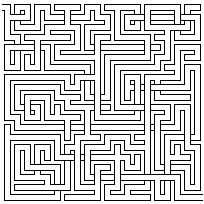
\includegraphics[width=4.094cm,height=4.094cm]{image/labyrinthe.png}}
\end{center}
	

%====================
\section{Définition}
%====================

	\textit{Le \textbf{backtracking} (appelé aussi \textbf{retour sur trace}) 
	est un algorithme qui consiste à revenir légèrement en arrière 
	sur des décisions prises afin de sortir d'un blocage. 	
	La méthode des essais et erreurs constitue un exemple simple de backtracking. 
	Le terme est surtout utilisé en programmation, où il désigne une stratégie 
	pour trouver des solutions à des problèmes de satisfaction de contraintes.} 
	(Wikipédia, août 2013)
	
	Le \textbf{backtracking} s'applique lorsque
	
	\begin{itemize}
		\item {
			Le problème à résoudre est fait d'une suite d'étapes.}
		\item {
			À chaque étape, plusieurs choix sont possibles 
			sans qu'il soit possible de «~calculer~» le bon.}
	\end{itemize}
	
	Pour \textbf{résoudre un tel problème}, il faudra procéder par essais.

	\begin{itemize}
		\item {
			Si, à une certaine étape, on arrive à une impasse, 
			il faudra revenir en arrière et remettre en doute un choix
			précédent.}
		\item {
			Il faudra bien sûr être précis pour être sûr 
			de tout tenter une et une seule fois.}
	\end{itemize}
	
	Un \textbf{exemple} courant est celui du \textbf{labyrinthe} 
	dont il faut trouver une sortie.

	\begin{itemize}
		\item {
			Il est formé de couloirs et de carrefours. 
			À chaque carrefour il faut faire un choix.}
		\item {
			Si on arrive à une impasse ou si on revient à un endroit déjà visité, 
			le chemin n'est pas le bon. Il faut revenir sur ses pas et 
			faire un autre choix à un carrefour (il faut s'assurer d'explorer 
			toutes les voies une et une seule fois).}
	\end{itemize}


%===========================================
\section{Structure générale de l'algorithme}
%===========================================

	\subsection{Pour obtenir une solution}
	%=====================================
		
		L'algorithme type pour résoudre un tel problème est toujours 
		le même. Seules quelques parties (en italique ci-dessous)
		devront être adaptées en fonction du problème précis.
		
		\cadre{
			\begin{pseudo}
				\Module{backtracking}{\textit{solution en construction}, ...}{booléen}
					\Decl réussite~: booléen
					\Let réussite \Gets faux
					\Stmt \textit{Initialiser les voies de recherche}
					\Repeat 
						\Stmt \textit{Choisir une voie non encore choisie}
						\If{\textit{la voie est acceptable}}
							\Stmt \textit{L'ajouter à la solution en cours}
							\If{\textit{la solution est incomplète}}
								\Let réussite \Gets backtracking(\textit{solution en construction}, ...)
								\If{NON réussite}
									\Stmt \textit{Enlever cette voie de la solution}
								\EndIf
							\Else
								\Let réussite \Gets vrai
							\EndIf
						\EndIf
					\Until{réussite OU \textit{toutes les voies ont été explorées} }
					\Return réussite
				\EndModule
			\end{pseudo}
		}

		Les questions fondamentales auxquelles 
		il faut répondre dans un cas précis sont~:

		\begin{enumerate}
			\item {
				À quoi correspond une étape ? 
				Quelles sont les voies possibles à chaque étape ?}
			\item {
				Comment représenter la solution en cours de construction ?}
			\item {
				Comment examiner toutes les voies possibles ? 
				Quand une voie est-elle acceptable ?}
		\end{enumerate}

	\subsection{Et pour obtenir toutes les solutions ?}
	%==================================================

		Avec l'algorithme précédent, on s'arrête quand on trouve UNE solution. 
		Comment faire si on veut TOUTES les solutions~? 
		Dans ce cas, la variable «~réussite~» n'est plus d'aucune utilité. 
		Quand une solution est complète, on peut la traiter (l'afficher ou 
		la sauver quelque part) et enlever le dernier morceau de la solution.

		\cadre{
			\begin{pseudo}
				\Module{backtracking}{\textit{solution en construction}, ...}{}
					\Stmt \textit{Initialiser les voies de recherche}
					\Repeat 
						\Stmt \textit{Choisir une voie non encore choisie}
						\If{\textit{la voie est acceptable}}
							\Stmt \textit{L'ajouter à la solution en cours}
							\If{\textit{la solution est incomplète}}
								\Stmt backtracking(\textit{solution en construction}, ...)
							\Else
								\Stmt \textit{On a une solution, la traiter}
							\EndIf
							\Stmt \textit{Enlever cette voie de la solution}
						\EndIf
					\Until{\textit{toutes les voies ont été explorées} }
				\EndModule
			\end{pseudo}
		}


%==================================
\section{Un exemple~: les 8 reines}
%==================================

	Il s'agit d'un exemple classique pour présenter le backtracking~: 
	Peut-on placer 8 reines sur un échiquier de  manière à ce qu'elles 
	ne soient pas en prise mutuellement?

	Aux échecs les reines se déplacent d'un nombre de 
	cases quelconque en ligne droite mais aussi en diagonale.

	\subsection{Étapes et voies de recherche}
	%========================================

	À chaque étape, on va placer une reine. Il n'est pas difficile 
	de se rendre compte que dans la solution, si elle existe,
	chaque reine est placée dans une ligne différente. Dès lors, 
	à chaque étape la ligne est fixée et il reste à choisir la
	colonne.

	\subsection{Comment représenter la solution ?}
	%=============================================

		La solution peut simplement être représentée par un tableau 
		de 8 entiers indiquant la colonne où se trouve la reine de
		la ligne $i$.

		\begin{itemize}
			\item {
				cols~: tableau de 8 entiers ($cols[i]$ indique 
				la colonne de la reine en ligne $i$)}
			\item {
				$ligne$~: entier indiquant la ligne de la reine suivante à placer}
		\end{itemize}
		
	\subsection{Quelles sont les voies à explorer ?}
	%===============================================

		À l'étape i, on l'a dit, on va ajouter la reine de la ligne $i$. 
		Les possibilités sont toutes les cases de cette ligne
		(toutes les colonnes donc). Un simple compteur permettra de 
		savoir où l'on en est. Une reine pourra être placée dans une
		case donnée si elle n'entre pas en conflit avec les reines 
		déjà placées jusqu'ici (elle ne peut être ni dans la même
		colonne ni dans la même diagonale)

	\subsection{La solution}
	%=======================

		\cadre{
			\begin{pseudo}
				\Module{huitReines}{}{}
					\Decl cols~: tableau [1 à 8] d'entiers
					\Stmt backtracking(cols, 1)
					\Stmt afficher(cols)
				\EndModule
			\end{pseudo}
		}
		
		\cadre{
			\begin{pseudo}
				\Module{bactracking}{cols\InOut~: tableau [1 à 8] d'entiers, ligne~: entier}{booléen}
					\Decl réussite~: booléen
					\Decl colonne~: entier
					\Let réussite \Gets faux
					\Let colonne \Gets 0
					\Repeat
						\Let colonne \Gets colonne + 1
						\If{estAcceptable(cols, ligne, colonne)}
							\Let cols[ligne] \Gets colonne
							\If{ligne<8}
								\Let réussite \Gets backtracking(cols, ligne+1)
								\LComment rien à faire si pas réussi, le choix suivant va écraser celui-ci.
							\Else 
								\Let réussite \Gets vrai
							\EndIf
						\EndIf
					\Until{réussite OU colonne = 8}
					\Return réussite
				\EndModule
			\end{pseudo}
		}
		
		\cadre{
			\begin{pseudo}
				\Module{estAcceptable}{cols~: tableau [1 à 8] d'entiers, ligne, colonne~: entier}{booléen}
					\Decl i~: entier
					\For{i \K{de} 1 \K{à} ligne-1}
						\If{cols[i] = colonne} 
							\Return faux
						\EndIf
						\If{ligne-i={\textbar}cols[i] - colonne{\textbar}}
							\Return faux
						\EndIf
					\EndFor
					\Return vrai
				\EndModule
			\end{pseudo}
		}
		
		
%======================================
\section{Autre exemple~: les cavaliers}
%======================================

	Encore un grand classique et toujours avec un échiquier. 
	Un cavalier peut-il se déplacer sur un échiquier de manière à
	passer sur toutes les cases une et une seule fois ?

	Un cavalier se déplace en «~L~». Il avance de 2 cases 
	en ligne droite puis tourne d'une case à droite ou à
	gauche.

	\subsection{Étapes et voies de recherche}
	%========================================

		Chaque étape correspond à un déplacement du cavalier. Il y aura 
		à chaque fois 8 destinations possibles (pour autant que
		cette case soit bien dans le plateau et qu'on n'y soit pas encore passé).

	\subsection{Comment représenter la solution ?}
	%=============================================

		Puisqu'il s'agit de déterminer les cases par lesquelles passe 
		le cavalier, on peut imaginer un tableau 8x8 d'entiers
		indiquant l'ordre de passage du cavalier par cette case. 
		Un 0 indiquera que le cavalier n'est pas encore passé par là.
		À chaque étape on remplit une case du tableau (on aura besoin 
		d'un compteur). La solution est finie quand tout le
		tableau est rempli (le compteur nous le dit facilement).

		\begin{itemize}
			\item {
				échiquier~: tableau 8x8 d'entiers initialisés à 0}
			\item {
				numéroEtape~: entier initialisé à 1}
		\end{itemize}
		
	\subsection{Quelles sont les voies à explorer ?}

		Simplement les cases vers lesquelles peut se déplacer le 
		cavalier. Mais comment facilement les trouver ? Le plus simple
		est d'utiliser deux tableaux reprenant les «~deltas~» (le nombre 
		de cases de déplacement en ligne et en colonne). Il vaut

		\begin{center}
			\tablefirsthead{\hline
			\centering{ \textsf{$\Delta L$}} &
			\centering{ -2} &
			\centering{ -2} &
			\centering{ -1} &
			\centering{ 1} &
			\centering{ 2} &
			\centering{ 2} &
			\centering{ 1} &
			\centering\arraybslash{ -1}\\}
			\tablehead{\hline
			\centering{ \textsf{$\Delta L$}} &
			\centering{ -2} &
			\centering{ -2} &
			\centering{ -1} &
			\centering{ 1} &
			\centering{ 2} &
			\centering{ 2} &
			\centering{ 1} &
			\centering\arraybslash{ -1}\\}
			\tabletail{}
			\tablelasttail{}
			\begin{supertabular}{|m{1.306cm}|m{0.379cm}|m{0.379cm}|m{0.379cm}|m{0.23900001cm}|m{0.23900001cm}|m{0.379cm}|m{0.379cm}|m{0.37300003cm}|}
			\hline
			\centering{ \textsf{$\Delta C$}} &
			\centering{ -1} &
			\centering{ 1} &
			\centering{ 2} &
			\centering{ 2} &
			\centering{ 1} &
			\centering{ -1} &
			\centering{ -2} &
			\centering\arraybslash{ -2}\\\hline
			\end{supertabular}
		\end{center}
		
		Un simple compteur permet de savoir où on en est dans cette exploration.

	\subsection{La solution}
	%=======================

		\cadre{
			\begin{pseudo}
				\Module{cavalier}{ligne, col~: entiers}{} 
				\RComment la position de départ
					\Decl \textsf{$\Delta L$}, \textsf{$\Delta C$}~: tableau [1 à 8] d'entiers 
					\RComment (initialisés comme ci-dessus)
					\Decl échiquier~: tableau [1 à 8, 1 à 8] d'entiers (initialisés à 0)
					\Let échiquier[ligne,col] \Gets 1
					\Stmt backtracking (échiquier, 2, ligne, {dots}, \ \textsf{$\Delta L$}, \textsf{$\Delta C$})
					\Stmt afficher(échiquier)
				\EndModule
			\end{pseudo}
		}
		
		\cadre{
			\begin{pseudo}
				\Module{bactracking}{échiquier\InOut~: tableau [1 à 8, 1 à 8] d'entiers, 
				numéroEtape, ligne, col~: entiers, \textsf{$\Delta L$}, 
				\textsf{$\Delta C$}~: tableau [1 à 8] d'entiers}{booléen}
					\Decl réussite~: booléen
					\Decl nouvelleLigne, nouvelleCol, numéroVoie~: entier
					\Let réussite \Gets faux
					\Let numéroVoie \Gets 0
					\Repeat
						\Let numéroVoie \Gets numéroVoie + 1
						\Let nouvelleLigne \Gets ligne + \textsf{$\Delta L$}[numéroVoie]
						\Let nouvelleCol \Gets col + \textsf{$\Delta C$}[numéroVoie]
						\If{estAcceptable(échiquier, nouvelleLigne, nouvelleCol)}
							\Let échiquier[nouvelleLigne, nouvelleCol] \Gets numéroEtape
							\If{numéroEtape<64}
								\Let réussite \Gets backtracking( échiquier, numéroEtape+1, nouvelleLigne, nouvelleCol, \ \textsf{$\Delta L$}, \textsf{$\Delta C$})
								\If{NON réussite}
									\Let échiquier[nouvelleLigne, nouvelleCol] \Gets 0
								\EndIf
							\Else
								\Let réussite \Gets vrai
							\EndIf
						\EndIf
					\Until{réussite ou numéroVoie=8}
					\Return réussite
				\EndModule
			\end{pseudo}
		}
		
		\cadre{
			\begin{pseudo}
				\Module{estAcceptable}{échiquier~: tableau [1 à 8, 1 à 8] d'entiers, nouvelleLigne, nouvelleCol~: entier}{booléen}
					\Return {1${\leq}$nouvelleLigne ET nouvelleLigne${\leq}$8 
					ET 1${\leq}$nouvelleCol ET nouvelleCol${\leq}$8 
					ET échiquier[ nouvelleLigne , nouvelleCol ] = 0}
				\EndModule
			\end{pseudo}
		}
		
		
%==================
\section{Exercices}
%===================

	\begin{Exercice}{La chaine}
		Construire une chaine de 100 occurrences des caractères 
		'A', `B' et `C' de manière à ce qu'il n'y ait jamais de
		sous-chaines adjacentes de mêmes longueurs qui soient identiques.

		\textbf{Exemples~: }

		\begin{itemize}
			\item {
				\underline{A\textbf{A}}BC est incorrect, A\underline{BC\textbf{BC}} aussi}
			\item {
				ABCBACAB est ok (mais pas 100)}
		\end{itemize}
	\end{Exercice}
	
	\begin{Exercice}{Carré magique}
		Un carré magique est un carré 3x3 rempli avec les nombres de 1 à 9 
		(une et une seule fois chacun) de telle façon que la
		somme de chaque ligne, de chaque colonne et de chaque diagonale 
		soit égale à 15. Écrivez un algorithme qui calcule
		toutes les solutions.
	\end{Exercice}
	
	\begin{Exercice}{Sudoku}
		\begin{enumerate}
			\item {
				Écrire un algorithme qui résout une grille de Sudoku. 
				À vous de décider comment représenter la grille de départ.}
			\item {
				Idem avec un Sudoku de type «~killer~» \newline
				(cf. \url{http://en.wikipedia.org/wiki/Killer_sudoku} pour une explication).
				
				Une grosse partie de la difficulté ici est de représenter correctement le problème.}
		\end{enumerate}
	\end{Exercice}
	
	\begin{Exercice}{Tetravex}
		\textit{«~Tetravex est un jeu de réflexion de type puzzle. Au début 
		du jeu, on commence avec une grille de taille 3*3 (par défaut) vierge, 
		et neuf carrés, ayant chacun un numéro sur chaque bord (donc quatre 
		numéros par carré). Le but est de	placer ces carrés sur la grille, 
		en faisant en sorte que le numéro d'un bord soit le même que 
		celui du carré adjacent.
		Chaque face de chaque carré est donc posée à coté d'une face 
		de même nombre. Le jeu est terminé quand la grille est
		remplie avec tous les carrés, correctement placés.~»} 
		(Wikipédia, août 2013)

		\begin{center}
			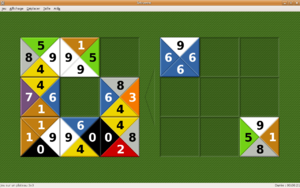
\includegraphics[width=7.938cm,height=4.974cm]{image/Backtracking-img002.png}
		\end{center}
		
		Écrivez un algorithme pour résoudre un tel problème.

		On suppose qu'on dispose d'une énumération pour les directions cardinales~:

		\cadre{
			\begin{pseudo}
				\Stmt \K{Énumération} Direction~: NORD, {dots}, SUD, OUEST
			\end{pseudo}
		}

		Ainsi qu'une classe pour représenter une pièce~:

		\cadre{
			\begin{pseudo}
				\Class{Pièce}
					\Public 
						\MethodSign{getValeur}{direction~: Direction}{entier}
				\EndClass
			\end{pseudo}
		}

		Écrire le module~:

		\cadre{
			\begin{pseudo}
				\ModuleSign{remplirGrille}{pièces~: tableau [1 à 9] de Pièce}{tableau [1 à 3, 1 à 3] de Pièce}
			\end{pseudo}
		}
	\end{Exercice}
		
	\begin{Exercice}{Le compte juste}
		
		Écrire un module retournant un booléen exprimant 
		le fait qu'une somme à payer peut être fournie 
		exactement avec les billets et la monnaie dont on dispose.
		
		\cadre{
			\begin{pseudo}
				\ModuleSign{compteJuste}{somme~: entier, disponible~: tableau [1 à n] d'entiers}{booléen}
			\end{pseudo}
		}
		
		Chaque entier du tableau représente la valeur d'une 
		pièce de monnaie ou d'un billet du portefeuille.

		\textbf{Exemple:~} 
		Avec les billets et pièces~: [ 10, 20, 50, 50, 5, 20, 2, 10, 10, {dots}, 
		peut-on payer 123 {\texteuro} ?
		
		Y a-t-il une autre façon de présenter les données 
		qui permettrait une optimisation de la recherche~?
	\end{Exercice}
	
	\begin{Exercice}{Le mot le plus long}
		Écrire un programme qui trouve tous les mots les plus 
		longs que l'on peut former à partir d'un ensemble de lettres.
		
		\cadre{
			\begin{pseudo}
				\ModuleSign{motsLesPlusLong}{lettres~: tableau [1 à n] de caractères}{}
				\LComment Affiche TOUS les mots les plus longs qu'on peut former avec les lettres données.
			\end{pseudo}
		}

		La classe Dictionnaire qui connait tous les mots valides est donnée.
		
		\cadre{
			\begin{pseudo}
				\Class{Dictionnaire}
					\Public 
						\ConstrSign{Dictionnaire}{}
						\LComment crée un dictionnaire avec tous les mots valides.
						\MethodSign{contientMot}{mot: chaine}{booléen}
						\LComment vrai si le mot est présent dans le dictionnaire.
						\MethodSign{contientMotCommencantPar}{mot: chaine}{booléen}
						\LComment vrai si le dictionnaire contient un mot commençant par la chaine donnée.
				\EndClass
			\end{pseudo}
		}
		
	\end{Exercice}
		